\chapter{Mesures}
\section{Introduction}
La théorie de la mesure, telle que présentée dans ce texte, est introduite comme
base du calcul intégral. Suivant l'approche historique de Lebesgue, elle
apparaît comme un cadre naturel pour définir une notion généralisée de longueur
ou de volume en dimension supérieure à 1. Pour préciser un peu mieux ce que l'on
entendra dans la suite par mesure, le cas du calcul de l'aire sous-tendue au
graphe d'une application réelle va être étudié plus avant. On supposera donnée
une application $f \colon [a,b] \to \mathbb{R}^+$, et on cherchera à déterminer
la surface de la partie $$\mathcal{D} = \{ (x,y) \in \mathbb{R}^2, \, x \in
[a,b], y \in [0, f(x)] \}$$ ainsi que représenté figure \ref{fig:01_01}.
\begin{figure}
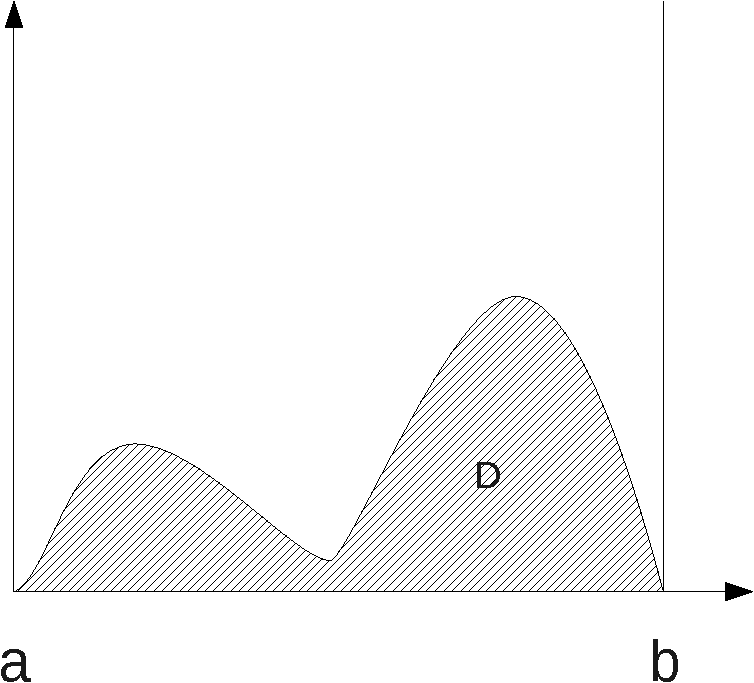
\includegraphics[scale=0.4]{images/surface_graphe.pdf}
\caption{Aire définie par un graphe d'application}\label{fig:01_01}
\end{figure}
L'aire de $\mathcal{D}$ peut être estimée en effectuant un découpage en
morceaux géométriquement simples (i.e. pour lesquels une aire peut facilement
être calculée) puis en sommant les différentes valeurs obtenues. Deux types de
découpages simples correspondant à des tranches verticales (resp. horizontales)
sont reproduits sur les figures \ref{fig:01_02}.

\begin{figure}
\begin{tabular}{cc}
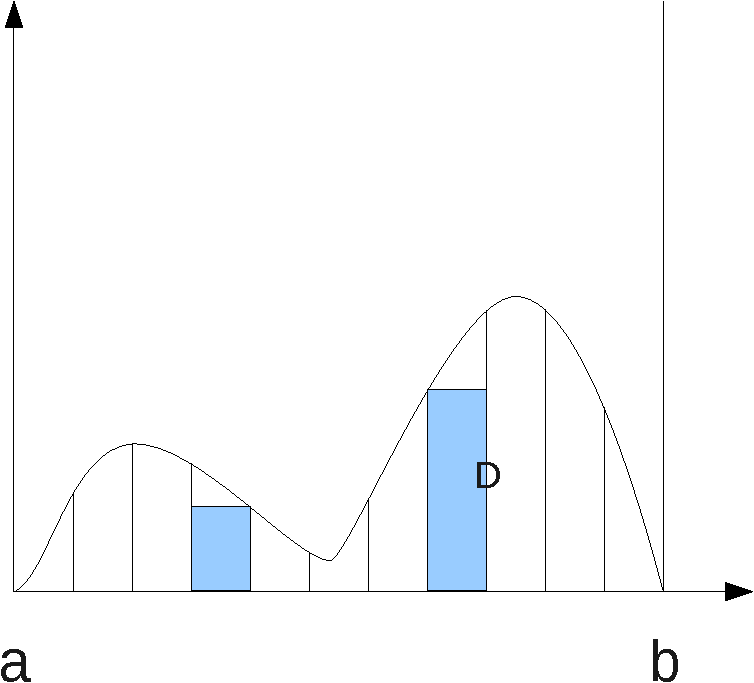
\includegraphics[scale=0.4]{images/graphe_riemann.pdf} & 
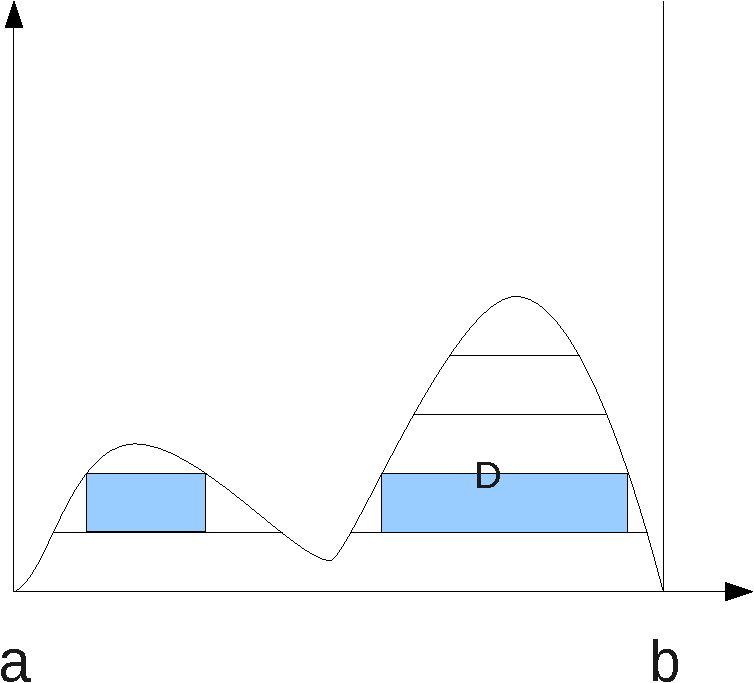
\includegraphics[scale=0.4]{images/graphe_lebesgue.pdf}
\end{tabular}
\caption{Découpages de Riemann et Lebesgue}\label{fig:01_02}
\end{figure}
Ces deux découpages vont correspondre dans la suite à deux notions
d'intégrales.

\subsection{Intégrale de Riemann}
L'estimation de la surface $\mathcal{D}$ à partir de bandes verticales est à la
base de la notion d'intégrale au sens de Riemann, qui est historiquement la
première à avoir été introduite. Ce découpage présente l'avantage considérable
de n'utiliser que des rectangles pour estimer l'aire de $\mathcal{D}$. Etant
donnée une subdivision $\mathcal{S}= \{ a = t_0 < t_1 < \dots < t_N = b \}$ de
l'intervalle $[a,b]$, et des points $\xi_i \in [t_i, t_{i+1}[, i = 0, \dots
,N-1$, une estimation de l'aire de $\mathcal{D}$ s'obtient à partir de
rectangles de base $[t_i, t_{i+1}]$ et de hauteur $f(\xi_i)$ comme:
\[
\mathcal{I}(\mathcal{S}, (\xi_i), f) =\sum_{i=0}^{N-1}
f(\xi_i)(t_{i+1}-t_i) \] $\mathcal{I}(\mathcal{S}, (\xi_i), f)$ est appelé somme
de Riemann de $f$ relative à la subdivision $\mathcal{S}$. Pour une subdivision
$\{ a = t_0 < t_1 < \dots < t_N = b \}$ donnée, les différentes sommes de Riemann
possibles différent par le choix des points d'évaluation $\xi_i, i=0 \dots N-1$.
Afin de pouvoir dégager une notion d'aire, il faut s'assurer de l'existence
d'une valeur limite aux sommes de Riemmann. La situation est un peu plus
compliquée que dans le cas des suites, l'ensemble des subdivisions sur un
intervalle donné n'étant pas dénombrable. La notion de filtre permet de
contourner le problème de façon élégante, mais on peut ici recourir à un
traitement plus simple. 
\begin{defn}
Soient  $\mathcal{S}_1= \{ a = t_0 < t_1 < \dots < t_N =
b \}$  et $\mathcal{S}_2= \{ a = u_0 < u_1 < \dots < u_M =
b \}$ deux subdivisions de $[a,b]$. On dira que $\mathcal{S}_2$ est plus fine
que $\mathcal{S}_1$, que l'on notera $\mathcal{S}_1 \prec \mathcal{S}_2$, si
$\mathcal{S}_1 \subset \mathcal{S}_2$.
\end{defn}

\begin{prop}\label{prop:union_subdivisions}
Pour tout couple de subdivisions $(\mathcal{S}_1,\mathcal{S}_2)$ de $[a,b]$, il
existe une subdivision $\mathcal{S}$ telle que $\mathcal{S}_1 \prec \mathcal{S}$
et $\mathcal{S}_2 \prec \mathcal{S}$
\end{prop}
\begin{proof}
Il suffit de poser $\mathcal{S}=\mathcal{S}_1 \cup \mathcal{S}_2$
\end{proof}

\begin{defn}\label{def:lim_riemann}
On dira que les sommes de Riemann de $f$ convergent vers une limite $l$ si pour
tout $\epsilon > 0$ il existe une subdivision $\mathcal{S}_{\epsilon}$ telle que
pour toute subdivision $\mathcal{S}=\{ a = t_0 < t_1 < \dots < t_N =
b \}$ plus fine que $\mathcal{S}_{\epsilon}$ et toute suite de points $\xi_i \in
[t_i, t_{i+1}[, \, i=0 \dots N-1$:
\[
|\mathcal{I}(\mathcal{S}, (\xi_i), f)-l| < \epsilon
\]
\end{defn}
La limite ainsi définie est unique. Supposons en effet l'existence d'une autre
valeur limite $l^\prime$ vérifiant la même propriété. Soit $\epsilon > 0$. Il
existe une subdivision $\mathcal{S}$ et une subdivision $\mathcal{S}^\prime$
telles que $|\mathcal{I}(\mathcal{S}, (\xi_i), f)-l| < \epsilon$,
$|\mathcal{I}(\mathcal{S^\prime}, (\xi^\prime_i), f)-l^\prime| < \epsilon$, les
mêmes inégalités étant vérifiées par toute subdivision plus fine. Par la
proposition \ref{prop:union_subdivisions}, il existe une subdivision
$\mathcal{U}$ plus fine que $\mathcal{S}$ et $\mathcal{S}^\prime$. Toute somme
de Riemann $\mathcal{I}(\mathcal{U}, (\theta_i), f)$ associée à $\mathcal{U}$
verifiera:
\[
|\mathcal{I}(\mathcal{U}, (\theta_i), f)-l| < \epsilon, \quad
|\mathcal{I}(\mathcal{U}, (\theta_i), f)-l^\prime| < \epsilon
\]
L'inégalité triangulaire montre alors que $|l-l^\prime|<2\epsilon$ et comme ceci
est vrai pour tout $\epsilon >0$, on en déduit $l=l^\prime$.
Le critère de Cauchy s'étend à la notion de limite indexée par des subdivisions. 
Enfin, si l'on se donne une subdivision $\mathcal{S}=\{ a = t_0 < t_1 < \dots <
t_N = b \}$, la quantité $\delta_{\mathcal{S}} = \sup \{ t_{i+1}-t_i, \,
i=0\dots N-1$ est appelée pas de $\mathcal{S}$. Si $\mathcal{S} \prec
\mathcal{S}^\prime$, alors $\delta_{\mathcal{S}^\prime} < \delta_{\mathcal{S}}$.
De plus, en choisissant des subdivisions de plus en plus fines, on peut faire
tendre le pas vers 0: ceci justifie l'abbréviation ''lorsque le pas des
subdivisions tend vers 0'' pour décrire la convergence des sommes de Riemann.

La valeur limite $l$ dans la définition \ref{def:lim_riemann}, lorsqu'elle
existe, est l'intégrale de Riemann de $f$ sur l'intervalle $[a,b]$ que l'on note
conventionnellement $\int_a^b f(t)dt$. Le point critique pour l'intégrabilité au
sens de Riemann est l'indépendance du choix des points $\xi_i$:
ceci impose une condition relativement forte sur le comportement local des
applications, comme le montre la proposition suivante.
\begin{prop} 
Soit $f \colon [a,b] \to \mathbb{R}^+$ telle qu'en tout
point de $]a,b[$, $f$ admette une limite à droite et à gauche, ainsi qu'une
limite à gauche (resp. à droite) en $b$ (resp. $a$). Alors $f$ est intégrable au
sens de Riemann.
 \end{prop}
 \begin{proof}
 L'idée de la preuve est résumée sur la figure \ref{fig:01_04}. Soit
 $\epsilon > 0$. Pour tout $t \in [a,b]$, il existe un intervalle ouvert
 (pour la topologie induite) $V_t = [a,b] \cap ]t-\eta_1, t+\eta_2[$  tel que
 $\forall x \in V_t, x < t$ (resp. $\forall x \in V_t, x > t$), $|f(x)
 -f(t^-)|<\epsilon$ (resp. $|f(x)-f(t^+)|<\epsilon$). L'intervalle $[a,b]$ étant compact, 
 un nombre fini de ces ouverts le recouvre ; on les notera $V_{t_i}, i = 0,
 \dots, N$.  Sans perte de généralité, on supposera que chaque intervalle
 contient un unique point $t_i$ de la subdivision et on posera $\theta = \inf \{
 t_{i+1}-t_i, i=0, \dots, N-1 \}$ . On peut déduire de l'écriture précédente l'existence d'une borne pour $f$, i.e. $\exists M >0, \, \forall x \in [a,b],
 |f(x)|\leq M$. Soient deux subdivisions $\mathcal{S}_1=\{x_0 < \dots <
 x_{N_1}\}$, $\mathcal{S}_2 = \{ y_0 < \dots < y_{N_2} \}$ de pas inférieur à
 $\theta$ et deux suites de points $(\xi_i)_{i=0, \dots, N_1 -1}$,
 $(\xi_j^\prime)_{j=0, \dots, N_2-1}$ vérifiant $\forall i=0, \dots, N_1-1,
 \xi_i \in [x_i, x_{i+1}[$ (resp. $\forall j=0, \dots, N_2-1,
 \xi_j^\prime \in [y_j, y_{j+1}[$). On posera $(z_k)_{k=0, \dots, N_3}$ la
 suite ordonnée obtenue à partir de l'ensemble $\{x_i,y_j, \,
 i=0,\dots,N_1 \,,  j=0, \dots, N_2 \}$ et $(\eta_k)_{k=0,\dots,N_3}$ (resp.
 $(\eta_k^\prime)_{k=0,\dots,N_3}$) la suite telle que $\eta_k = \xi_i \text{ si
 } [z_k, z_{k+1}[ \subset [x_i, x_{i+1}[$ (resp. $\eta_k^\prime = \xi_j^\prime
 \text{ si } [z_k, z_{k+1}[ \subset [y_j, y_{j+1}[$).
 On a:
 \begin{align*}
  & |\mathcal{I}(\mathcal{S}_1, (\xi_i), f) -\mathcal{I}(\mathcal{S}_2,
 (\xi^\prime_j), f)| = \\
 & \left|\sum_{i=0}^{N_1-1} f(\xi_i)(x_{i+1}-x_i) -
 \sum_{j=0}^{N_2-1}f(\xi_j^\prime)(y_{j+1}-y_j) \right| \leq \\
 & \sum_{k=0}^{N_3} |f(\eta_k)-f(\eta_k^\prime)|(z_{k+1}-z_k)
 \end{align*}
 Dans cette dernière somme, il existe $N$ indices $k$ tels que l'intervalle
 correspondant $[z_k, z_{k+1}[$ contienne exactement un des points $(t_i)_{i=0,
 \dots, N}$. Le terme correspondant se majore par $2Mh$ où
 $h=\sup(\delta(\mathcal{S}_1),\delta(\mathcal{S}_1))$. Pour tous les autres
 termes, $|f(\eta_k)-f(\eta_k^\prime)| < 2\epsilon$, ce qui donne au total la
 majoration:
 \[
 |\mathcal{I}(\mathcal{S}_1, (\xi_i), f) -\mathcal{I}(\mathcal{S}_2,
 (\xi^\prime_j), f)| \leq 2MNh + 2\epsilon(b-a)
 \]
 Si $h < \epsilon / N$, on obtient finalement:
  \[
 |\mathcal{I}(\mathcal{S}_1, (\xi_i), f) -\mathcal{I}(\mathcal{S}_2,
 (\xi^\prime_j), f)| \leq 2\epsilon(M +(b-a))
 \]
 ce qui montre que l'écart entre $\mathcal{I}(\mathcal{S}_1, (\xi_i), f)$ et $\mathcal{I}(\mathcal{S}_2,
 (\xi^\prime_j), f)$ peut être rendu aussi petit que l'on veut, indépendamment
 du choix des points $(\xi_i),(\xi_j^\prime)$, dès lors que les pas des
 subdivisions sont inférieurs à une valeur donnée. En vertu du critère de
 Cauchy, ceci implique l'existence de l'intégrale de Riemann de $f$.
 \end{proof}
 \begin{figure}
 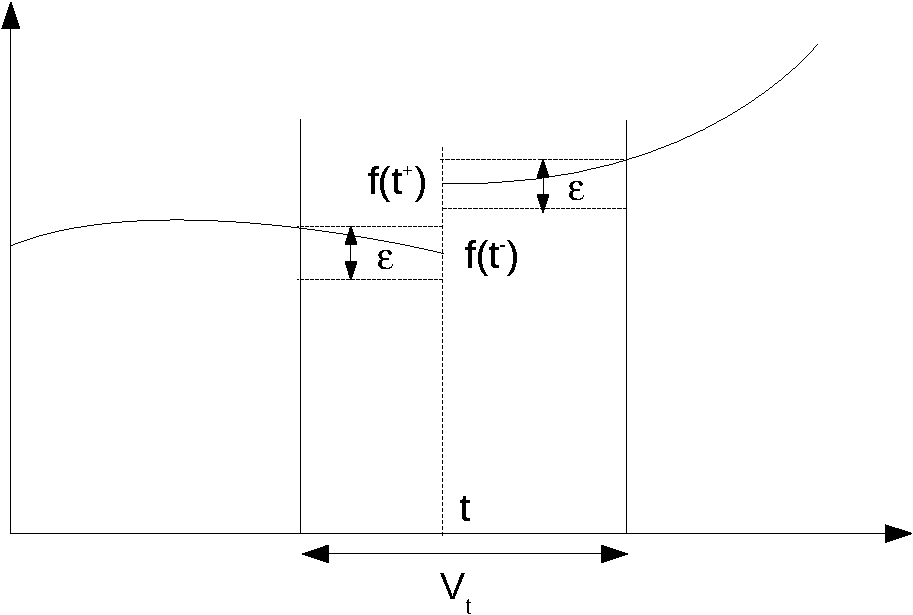
\includegraphics[scale=0.4]{images/fct_reglee.pdf}
 \caption{Encadrement de $f$ au voisinage d'un point $t$}\label{fig:01_04}
 \end{figure}
La preuve précédente dépend de façon critique du caractère compact de
l'intervalle $[a,b]$. L'extension à des domaines plus généraux ne pourra pas se
faire en utilisant le même procédé. De plus, on peut noter que la démonstration
qui vient d'être faite montre également que si une application $f$ vérifie les
hypothèse de la proposition, alors elle est limite uniforme d'applications en
escalier, qui sont définies comme suit:
\begin{defn}
Soit $[a,b]$ un intervalle compact. Une application $f \colon [a,b] \to
\mathbb{R}$ est dite en escalier si il existe une subdivision $a=t_0 < \dots <
t_N =b$ de $[a,b]$ telle que $f$ soit constante sur les intervalles
$]t_i,t_{i+1}[, i=0,\dots,N$.
\end{defn}
Ce qui implique aussi que $f$ ne peut avoir plus d'un nombre dénombrable de
points de discontinuité. 
On remarquera enfin, toujours en considérant la preuve effectuée, que
l'extension de l'intégrale de Riemann à des fonctions prenant leurs valeurs dans
un autre ensemble que $\mathbb{R}^+$ ne pose pas de problème dès lors qu'il
s'agit d'un espace topologique complet. Ceci explique pourquoi cette définition
de l'intégrale reste très utilisée. 

La difficulté majeure qui se pose avec l'intégration au sens de Riemann, et qui
a motivé en partie les travaux de Lebesgue, est la difficulté d'intervertir
limite et intégrale:
\begin{prop}
Soit $(f_n)_{n \in \mathbb{N}}$ une suite d'applications intégrables au sens de
Riemann et de limite uniforme $f$. Alors $f$ est intégrable au sens de Riemann
et:
\[
\int_a^b f(t) dt = \lim_{n \to +\infty} \int_a^b f_n(t)dt
\]
\end{prop}
\begin{proof}
Soit $\epsilon > 0$. Il existe $N_\epsilon \in \mathbb{N}$ tel que $\forall n
\geq  N_\epsilon$, $\sup_{x\in[a,b]} \left|f_n(x)-f(x)\right|<\epsilon$. Soit
$a=t_0<\dots<t_N=b$ une subdivision de $[a,b]$ et $(\xi_i)_{i=0,\dots, N-1}$ une
suite de points telle que $\xi_i \in [t_i,t_{i+1}[,i=0,\dots,N-1$. On a, pour
$n \geq N_\epsilon$:
\begin{align*}
& \left|\sum_{i=0}^{N-1}f(\xi_i)(t_{i+1}-t_i) -
\sum_{i=0}^{N-1}f_n(\xi_i)(t_{i+1}-t_i)\right|\\
& \leq
\sum_{i=0}^{N-1}\left|f(\xi_i)-f_n(\xi_i)\right|(t_{i+1}-t_i) \\
& \leq \epsilon(b-a)
\end{align*}
On en déduit que pour deux subdivisions $\mathcal{S}_1$, $\mathcal{S}_2$ et
deux suites associées $(\xi_i), (\xi_j^\prime)$:
\begin{align*}
& |\mathcal{I}(\mathcal{S}_1, (\xi_i), f) -\mathcal{I}(\mathcal{S}_2,
 (\xi^\prime_j), f) | \leq \\
 & |\mathcal{I}(\mathcal{S}_1, (\xi_i), f_n)
 -\mathcal{I}(\mathcal{S}_2, (\xi^\prime_j), f_n) | + 2 \epsilon (b-a)
\end{align*}
$f_n$ étant par hypothèse Riemann-intégrable, on a pour des subdivisions de
pas suffisamment petit:
\[
|\mathcal{I}(\mathcal{S}_1, (\xi_i), f) -\mathcal{I}(\mathcal{S}_2,
 (\xi^\prime_j), f) | \leq \epsilon(1 + 2 (b-a))
\]
En application du critère de Cauchy, on en déduit l'existence d'une limite à
$\mathcal{I}(\mathcal{S}, (\xi_i), f)$ lorsque le pas de la subdivision
$\mathcal{S}$ tend vers 0. L'égalité:
\[
\int_a^b f(t)dt = \lim_{n \to +\infty} \int_a^b f_n(t)dt
\]
s'obtient aisément.
\end{proof}
Il apparaît clairement dans cette preuve la nécessité de la convergence uniforme
afin de borner la différence entre une somme de Riemann de $f$ et de celle
de l'une des $f_n$: la convergence simple ne permet pas de conclure. 
Ce résultat montre également qu'il est possible de calculer l'intégrale de
Riemann d'une application à partir de la limite uniforme d'une suite
d'applications en escalier (voir plus haut). 

L'impossibilité de prendre une hypothèse plus faible que la convergence uniforme
résulte du découpage en tranches verticales choisi: il est nécessaire de
contrôler la hauteur du découpage, donc la valeur des fonctions sur tout un
intervalle. 

\subsection{Intégrale de Lebesgue}
Le second type de découpage definit par passage à la limite l'intégrale de
Lebesgue. Etant donné que les subdivisions effectuées se font sur l'ensemble des
valeurs de l'application, l'extension à des domaines généraux est relativement
aisée. De plus, pour la même raison, il ne sera pas nécessaire d'avoir
convergence uniforme pour conclure que l'intégrale d'une limite est la limite
des intégrales. La difficulté principale dans cette procédure réside dans le
fait qu'il est nécessaire de pouvoir définir la longueur d'une image réciproque
d'intervalle, qui n'a aucune raison d'être un intervalle. La définition précise
de cette longueur généralisée est l'objet de la théorie de la mesure. On
supposera que l'on dispose d'une telle "longueur" qui à une partie $A \subset
\mathbb{R}$ associe un réel positif $\lambda(A)$. Soit $f\colon \mathbb{R}\to
 \mathbb{R}^+$ une application à valeurs positives. Soit $a>0$ fixé et $0=t_0 <
\dots < t_N = a$ une subdivision de l'intervalle $[0,a]$. Une estimation par
défaut de l'aire sous-tendue au graphe de $f$ est obtenue facilement par:
\[
\sum_{i=0}^{N-1} t_{i} \lambda(f^{-1}([t_i, t_{i+1}[)) + t_N
\lambda(f^{-1}([a, +\infty[))
\]
Si le  passage à la limite $a \to +\infty$, $N \to \infty$ est possible, la
valeur ainsi obtenue sera appelée intégrale de Lebesgue. On peut se poser la
question de l'existence de la limite en question et de savoir si la définition 
de la surface au sens de Lebesgue est compatible, au
moins sur une classe assez large de fonctions, avec l'intégrale de Riemann
précédente. 
En guise de préliminaire assez intuitif, il para\^{\i}t raisonnable d'imposer
que pour un intervalle $[a,b[$, la longueur $\lambda([a,b[)$ soit $b-a$. Ceci
permet d'ores et déjà le calcul de l'intégrale de Lesbesgue sur des fonctions en
escalier. Soit $f \colon [a,b] \to \mathbb{R}^+$ une telle application qui
admettra une expression:
\[
f = \sum_{i=0}^N a_i 1_{I_i}
\]
avec $I_i$ un intervalle $[c_i, c_{i+1}[$.
On note de façon usuelle $1_A$ pour une partie $A \subset \mathbb{R}$
l'application indicatrice de $A$:
\[
f \colon x \mapsto \left \{
\begin{array}{cc}
0 & x \notin A \\
1 & x \in A
\end{array} 
\right.
\]

$f$ prend ses valeurs dans le compact $[0,
\sup_{i=0,\dots ,N}a_i]$. Soit $a > \sup_{i=0,\dots ,N}a_i$ et $0 = t_0 < \dots
< t_M = a$ une subdivision de l'intervalle $[0,a]$ de pas inférieur à $\inf
\{a_{i+1}-a_i, \, i=0, \dots, N-1\}$. Tout intervalle de la subdivision contient
soit aucun soit un unique point $a_i$. On en déduit que pour tout $t_j$,
$f^{-1}([t_j, t_{j+1}[)$ est soit vide (donc de longueur nulle), soit une union
disjointes des intervalles associés à l'unique valeur $a_i$ qui se trouve dans l'intervalle $[t_j, t_{j+1}[$, ce qui donne: 
\[
\sum_{i=0}^{N-1} t_{i} \lambda(f^{-1}([t_i, t_{i+1}[)) + t_N
\lambda(f^{-1}([a, +\infty[)) = \sum_{i=0}^N a_i (c_{i+1} - c_i)
\]
Cette expression est la même que celle trouvée dans le cadre de la théorie de
Riemann et laisse à penser que les deux notions d'intégrales coïncideront au
minimum sur les applications continues (une telle application étant limite
uniforme d'applications en escalier).

Les rapides développements précédents montrent au moins intuitivement que la
définition de l'intégrale de Lebesgue sera particulièrement simple, toute la
difficulté étant reportée sur la notion de "longueur" qui sera dans la suite
appelée mesure, et sur la détermination des parties pouvant admettre une mesure.
\section{Algèbres et tribus de parties}
Les notions d'algèbres et de tribus de parties sont à la base de
la théorie de la mesure.
\begin{mandatory}
\begin{defn}
Soit $E$ un ensemble. Un ensemble de parties $\mathcal{T}$ de $E$ est
appelé algèbre de parties si les axiomes suivants sont vérifiés~:
\begin{itemize}
\item $E \in \mathcal{T}$.
\item $A \in \mathcal{T} \Rightarrow A^c \in \mathcal{T}$ où la
  notation $A^c$ désigne le complémentaire de $A$ dans $E$.
\item Pour tout suite finie $(A_i)_{i=0\dots n}$ d'éléments de
  $\mathcal{T}$, $\cap_{i=0\dots n }  A_i \in \mathcal{T}$.
\end{itemize}
\end{defn}
\end{mandatory}
On notera que les axiomes précédents impliquent également que
$\emptyset \in \mathcal{T}$ et que toute union finie d'éléments de
$\mathcal{T}$ est encore un élément de $\mathcal{T}$.

\begin{mandatory}
\begin{defn}
Soit $E$ un ensemble. Une tribu $\mathcal{T}$ est un
ensemble de parties de $E$ vérifiant les axiomes~:
\begin{itemize}
\item $E \in \mathcal{T}$.
\item $A \in \mathcal{T} \Rightarrow A^c \in \mathcal{T}$ où la
  notation $A^c$ désigne le complémentaire de $A$ dans $E$.
\item Pour tout suite dénombrable $(A_i)_{i \in \mathbb{N}}$ d'éléments de
  $\mathcal{T}$, $\cap_{i \in \mathbb{N}}  A_i \in \mathcal{T}$.
\end{itemize}
\end{defn}
\end{mandatory}
Toute tribu est une algèbre~: il suffit de  remarquer que le dernier
axiome peut aussi s'appliquer aux familles finies $(A_i)_{0=1\dots n}$
en considérant une suite stationnaire $(B_i)_{i  \in \mathbb{N}}$~:
\[
B_i = \left \{ \begin{array}{cc}
A_i & i \leq n \\
A_n & i > n
\end{array} \right .
\]
\begin{term}
  Une tribu de parties est aussi appelée $\sigma$-algèbre de
parties (la lettre $\sigma$ préfixant un objet indique généralement une
extension des lois définies sur cet objet à des famillles dénombrables). Les
parties d'une tribu $\mathcal{T}$ sont appelées parties $\mathcal{T}$-mesurables.
\end{term}
\begin{exemple}
Pour tout ensemble $E$, l'ensemble des parties de $E$ forme de façon
évidente une tribu, de même que $\{E, \emptyset\}$. Ces
tribus sont respectivement, au sens de l'inclusion,  la plus grande et la plus petite tribu qui puisse se
construire sur $E$.
\end{exemple}
\begin{exemple}
Dans un ensemble $E$, l'ensemble des parties dénomb\-rables ou de
complémentaire dénombrable est également une tribu. Pour
vérifier ceci, seul l'axiome concernant les intersections ou
réunions dénombrables mérite examen. Soit $(A_i)_{i \in \mathbb{N}}$
une famille de parties mesurables. Pour tout $i \in \mathbb{N}$, $A_i$
ou $A_i^c$ est dénombrable. Supposons dans un premier temps qu'il
existe un entier $i_0$ tel que $A_{i_0}$ soit dénombrable. Comme
$\cap_{i \in \mathbb{N}} A_i \subset A_{i_0}$, on en déduit que le
cardinal de l'intersection est dénombrable. Si on ne peut trouver de
$i_0$ vérifiant la propriété, alors tous les $A_i^c$ sont de cardinal
dénombrable. $\cup_{i \in \mathbb{N}} A_i^c$ est aussi dénombrable. Comme par
ailleurs $\cap_{i \in \mathbb{N}} A_i = \left (\cup_{i \in \mathbb{N}}
A_i^c \right ) ^c$, $\cap_{i \in \mathbb{N}} A_i$ est de
complémentaire dénombrable, ce qui termine la démonstration.
\end{exemple}
\begin{exemple}
Dans un ensemble $E$ de cardinal infini, l'ensemble des parties
de cardinal fini ou de complémentaire de cardinal fini forme une
algèbre de parties, mais n'est pas une tribu~: comme $E$
est de cardinal infini, il est possible de choisir une famille
dénombrable 
$(x_i)_{i \mathbb{N}}$ d'éléments distincts. La réunion $\cup_{i
\in \mathbb{N}} \{ x_i \}$ est une réunion dénombrable de parties de
cardinal fini mais n'est pas elle même de cardinal fini. Comme par
ailleurs il est possible de faire une partition de $E$ sous la forme
de deux ensembles infinis (considérer par exemple $E=\mathbb{N}$ et
les entiers pairs et impairs), on peut faire en sorte que le cardinal
de son complémentaire ne soit pas non plus fini. 
\end{exemple}
\begin{prop}
Soit $\mathcal{T}$ une algèbre de parties sur un ensemble $E$. Si pour toute
famille $(A_i)_{i \in \mathbb{N}}$ d'éléments de $\mathcal{T}$, croissante au
sens de l'inclusion, on a $\cup_{i \in \mathbb{N}} A_i \in \mathcal{T}$
alors $\mathcal{T}$ est une tribu. La proposition subsiste
si l'on remplace famille croissante par famille décroissante et
réunion par intersection.
\end{prop}
\begin{proof}
Il suffit de vérifier l'axiome relatif aux unions dénombrables. Soit
$(A_i)_{i \in \mathbb{N}}$ une famille d'éléments de $\mathcal{T}$. La
famille $B_n = \cup_{i=0}^n A_i$ est croissante au sens de
l'inclusion. $\mathcal{T}$ étant une algèbre par hypothèse, $B_n \in
\mathcal{T}$ pour tout entier $n$, d'où $\cup_{i \in \mathbb{N}} B_i =
\cup_{i \in \mathbb{N}} A_i \in \mathcal{T}$.
La proposition relative aux familles décroissantes s'obtient par
passage au complémentaire.
\end{proof}
\begin{rem}
Il est possible de trouver d'autres caractérisations équivalentes des
tribus. En particulier, si l'on impose à une algèbre
$\mathcal{T}$ d'être stable par union dénombrable {\em disjointe},
$\mathcal{T}$ est une tribu. En effet, si $(A_i)_{i \in
\mathbb{N}}$ est une famille disjointe d'éléments de $\mathcal{T}$, la
famille $B_n =  \cup_{i=0 \dots n} A_i$ est une famille croissante au
sens de l'inclusion d'éléments de $\mathcal{T}$ et la proposition
précédente s'applique. 
\end{rem}
\begin{mandatory}
\begin{prop}Soit $E$ un ensemble. Toute intersection de
  tribus sur $E$ est encore une tribu sur $E$.
\end{prop}
\end{mandatory}
\begin{proof}
$E$ appartient à l'intersection des tribus car il appartient par définition
à chacune des tribus. Soit $A$ une partie de l'intersection. $A$ appartient à toutes
les tribus de l'intersection. $A^c$ appartient aussi à toutes les tribus
de l'intersection, donc à l'intersection. Enfin, si $(A_i)_{i \in \mathbb{N}}$ est une famille de parties
appartenant chacune à l'intersection des tribus, $\cap_{i \in \mathbb{N}} A_i$ appartient à toutes
les tribus et donc à l'intersection.
\end{proof}
\leftline{\em Attention !}
La réunion d'algèbres n'est pas nécessairement une algèbre comme le
montre l'exemple ci dessous avec $E= \{ 0, 1, 2 \}$~:
\begin{align*}
&\mathcal{T}_1 = \{ \emptyset, \{ 0,1 \}, \{ 2\}, E \} \\
&\mathcal{T}_2 = \{ \emptyset, \{ 0\}, \{1, 2\}, E \} \\
& \mathcal{T}_1 \cup \mathcal{T}_2 = \{ \emptyset, \{ 0\}, \{ 2\},  \{ 0,1
\},\{1, 2\}, E \}
\end{align*}
$\mathcal{T}_1, \mathcal{T}_2$ sont des algèbres, mais $ \mathcal{T}_1
\cup \mathcal{T}_2$ ne contient pas $\{1\} = \{ 0,1 \} \cap \{1, 2\}$
et ne peut donc être une algèbre.

On notera le très important corollaire suivant~:
\begin{mandatory}
\begin{corollaire}
Soit $E$ un ensemble et $\mathcal{F}$ un ensemble de parties de
$E$. Il existe une unique plus petite tribu contenant
$\mathcal{F}$, appelée tribu engendrée par $\mathcal{F}$.
\end{corollaire}
\end{mandatory}
L'ensemble des tribus contenant $\mathcal{F}$ n'est pas
vide car $\mathcal{P}(E)$ est une tribu.
Il suffit alors de construire l'intersection de toutes les
tribus contenant $\mathcal{F}$, qui est une
tribu par le corollaire précédent. L'unicité provient de la
minimalité de la tribu engendrée. 
La tribu engendrée par $\mathcal{F}$ sera notée $\sigma(\mathcal{F})$.
\begin{mandatory}
\begin{defn}
Soit $E$ un ensemble muni d'une topologie $\mathcal{O}$. La plus
petite tribu sur $E$ contenant les ouverts de $
\mathcal{O}$ est appelée tribu de Borel relativement à la
topologie $\mathcal{O}$.
\end{defn}
\end{mandatory}
La tribu de Borel sur $E$ est notée $\mathcal{B}(E)$, la topologie
étant sous-entendue. La tribu de Borel sur $E$ est également engendrée
par les fermés. Les éléments de la tribu de Borel s'appellent les boréliens.
La tribu de Borel  sur $\mathbb{R}^n$ muni de
la topologie induite par la norme euclidienne est d'un usage constant
en théorie de l'intégration. Il existe plusieurs façons équivalentes
de la construire, esentiellement à partir d'ensembles de parties simples comme
va le montrer la proposition suivante.
\begin{mandatory}
\begin{prop}
 La tribu de Borel sur $\mathbb{R}^n$ muni de
la topologie induite par la norme euclidienne est égale à la tribu engendrée par l'une quelconque
des familles suivantes~:
\begin{itemize}
\item L'ensemble des ouverts (resp. fermés) de $\mathbb{R}^n$.
\item L'ensemble des demi-espaces de la forme~:
\[
H_{i,\lambda} = \{ (x_1, \dots x_n) | x_i < \lambda \} 
\]
avec $i \in 1 \dots n, \lambda \in \mathbb{R}$.
\item L'ensemble des rectangles~:
\[
\{ (x_1,\dots ,x_n) | a_i \leq  x_i < b_i, \, i=1\dots n \}
\]
\end{itemize}
\end{prop}
\end{mandatory}
\begin{proof}
Soit $\mathcal{B}_1$ la tribu engendrée par les
demi-espaces et $\mathcal{B}_2$ la tribu engendrée par les
rectangles. On a $\mathcal{B}_1 \subset \mathcal{B}(\mathcal{R}^n)$
car les demi-espaces sont des ouverts. Un rectangle quelconque pouvant
être obtenu par intersection finie de différences de demi-espa\-ces, on
en déduit que l'ensemble des rectangles est inclus dans
$\mathcal{B}_1$, et donc, par minimalité de la tribu engendrée, que
$\mathcal{B}_2 \subset \mathcal{B}_1$.
Enfin, soit $O$ un ouvert de $\mathbb{R}^n$. Il existe une famille
dénombrable $(x^{(i)}_{i \in \mathbb{N}})$ de points de $O$ et une famille
$(r_i)_{i \in \mathbb{N}}$ de réels positifs telles que~:
\[
O = \bigcup_{i \in \mathbb{N}} B(x^{(i)}, r_i)
\]
avec $B(x^{(i)}, r_i)$ boule ouverte de centre $x^{(i)}$ et de rayon
$r_i$. Les normes étant équivalentes sur $\mathbb{R}^n$, on 
choisira la norme sup:
$$\| x \| = sup_{i=1\dots n}
|x_i|$$
 pour laquelle les boules ouvertes sont des rectangles
ouverts. Comme par ailleurs~:
\begin{align*}
&\{ (x_1,\dots ,x_n) | a_i <  x_i < b_i, \, i=1\dots n \}  = \\
&\bigcup_{k \geq 1} \{ (x_1,\dots ,x_n) | a_i + \frac{1}{k} \leq  x_i < b_i, \,
i=1\dots n \}
\end{align*}
on peut obtenir $O$ par réunion dénombrable de rectangle
semi-ouverts. Ceci prouve que l'ensemble des ouverts est contenu dans
$\mathcal{B}_2$. Par ail\-leurs, on a de façon évidente $\mathcal{B}_1
\subset \mathcal{B}(\mathbb{R}^n)$, ce qui termine la proposition.
\end{proof}
\begin{exercice}
On se place dans l'ensemble des nombres entiers naturels $\mathbb{N}$. 
 \begin{itemize}
  \item Soit $n \in \mathbb{N}$ un entier fixé. Déterminer la tribu
  $\mathcal{T}_n$ engendrée par les singletons $\{0\},\{1\},\dots,\{n\}$.
  \item Montrer que pour tout $N \in \mathbb{N}$:
  \[
  	\bigcup_{n=0}^N \mathcal{T}_n
  \]
  est une tribu.
  \item Est-ce que:
    \[
  	\bigcup_{n=0}^{+\infty} \mathcal{T}_n
  \]
  est encore une tribu ?
\end{itemize}
\end{exercice}
\section{Mesures}
\subsection{La droite réelle achevée}
En théorie de la mesure, l'usage de la droite réelle complétée par les
points $\{+\infty, -\infty \}$ ou de la demi-droite achevée $[0,
+\infty]$ est courant. Dans ce paragraphe, les propriétés utiles de
ces objets vont être brièvement rappelées. Les démonstrations des
différentes propositions sont laissées au lecteur à titre d'exercice.
\begin{defn}
La droite réelle achevée, notée $\overline{\mathbb{R}}$, est l'ensemble
$\mathbb{R} \cup \{ -\infty, +\infty \}$ muni de la topologie
suivante~:
\begin{itemize}
\item Toute partie de $\overline{\mathbb{R}}$ ne contenant pas
$+\infty$ ou $-\infty$ est ouverte si et seulement si elle est ouverte
dans $\mathbb{R}$ muni de sa topologie usuelle.
\item Une partie de  $\overline{\mathbb{R}}$ est un voisinage de
$+\infty$ (resp. $-\infty$) si et seulement si elle contient un
intervalle de la forme $]A, +\infty] = \{+\infty\} \cup \{ x \in
\mathbb{R} | x > A \}$ (resp. $[-\infty, A[ = \{-\infty\} \cup \{ x \in
\mathbb{R} | x < A \}$).
\end{itemize}
\end{defn}
On munira $\overline{\mathbb{R}}$ des règles arithmétiques suivantes~:
\begin{itemize}
\item Les opérations entre éléments de $\mathbb{R}$ sont les
opérations usuelles.
\item Si $x \in \mathbb{R}$, $x+(+\infty) = (+\infty) + x = +\infty$,
$x+(-\infty) = (-\infty) + x = -\infty$.
\item Si $x \in \mathbb{R}, x > 0$, $x.(+\infty) = (+\infty).x = +\infty$,
$x.(-\infty) = (-\infty) . x = -\infty$.
\item  Si $x \in \mathbb{R}, x < 0$, $x.(+\infty) = (+\infty).x = -\infty$,
$x.(-\infty) = (-\infty) . x = +\infty$.
\item $(+\infty)+(+\infty) = +\infty$,  $(-\infty)+(-\infty) =
-\infty$.
\item $(+\infty).(+\infty) = +\infty$, $(-\infty).(-\infty) =
+\infty$, $(+\infty).(-\infty) = -\infty$, $0.(+\infty)=0.(-\infty)=0$.
\end{itemize}
Les opérations précédentes sont commutatives. La somme
$(+\infty)+(-\infty)$ n'est pas définie.
La valeur absolue de $\mathbb{R}$ se prolonge sur la droite achevée
par $|+\infty|=|-\infty|=+\infty$.
\begin{prop}
Toute partie $A \subset \overline{\mathbb{R}}$ admet une borne
supérieure notée $sup(A)$ et une borne inférieure notée $inf(A)$.
\end{prop}
La caractérisation suivante du $sup$ est très utile en pratique.
\begin{prop}
$\lambda \in \mathbb{R}$ est la borne supérieure de $A$ si~:
\begin{itemize}
\item $\forall x \in A, \, x \leq \lambda$.
\item $\forall \epsilon > 0, \exists y \in A | y > \lambda - \epsilon$.
\end{itemize}
$+\infty$ est la borne supérieure de $A$ si $\forall M \in
\mathbb{R}, \exists x \in A | x > M$. 
\end{prop}
Cette caractérisation se transpose de façon évidente à l'$inf$.
\begin{mandatory}
\begin{defn}
Soit $(x_n)_{n \in \mathbb{N}}$ une suite d'éléments de
$\overline{\mathbb{R}}$. La limite supérieure (resp. inférieure) de
cette suite, notée $\limsup_n x_n$ (resp. $\liminf_n x_n$), est~:
\[ \limsup_n x_n =\inf_{k \in \mathbb{N}} \sup_{n \geq k} x_n 
\]
resp.~:
\[ \liminf_n x_n = \sup_{k \in \mathbb{N}} \inf_{n \geq k} x_n
\]
 Une suite est dite convergente
si $\liminf_n = \limsup_n$ et la valeur commune est appelée limite de
la suite.
\end{defn}
\end{mandatory}
\begin{rem}
Les limites inférieure et supérieure, définies à partir des bornes
inférieures et supérieures existent toujours, contrairement à la
limite. Dans $\overline{\mathbb{R}}$, la limite d'une suite
convergente peut être $+\infty$ ou $-\infty$. On trouve quelquefois le
terme de suite divergente vers l'infini pour qualifier de telles suites.
\end{rem}
\subsection{Mesures positives}
\begin{defn}
Soit $E$ un ensemble et  $\mathcal{T}$ une tribu sur
$E$. Le couple $(E, \mathcal{T})$ est appelé espace mesurable. 
\end{defn}
\begin{mandatory}
\begin{defn}
Soit $(E, \mathcal{T})$ un espace mesurable. Une mesure sur cet espace
est une application $\mu : \mathcal{T} \to [0, +\infty]$ vérifiant~:
\begin{itemize}
\item $\mu(\emptyset) = 0$.
\item Pour toute suite $(A_i)_{i \in \mathbb{N}}$ d'éléments disjoints
  de  $\mathcal{T}$, on a~:
\[
\mu \left ( \cup_{i \in \mathbb{N}} A_i \right ) = \sum_{i
  =0}^{+\infty} \mu(A_i)
\]
\end{itemize}
\end{defn}
Le triplet $(E, \mathcal{T}, \mu)$ est appelé espace mesuré.
\end{mandatory} 

Voici quelques exemples de mesures usuelles~:
\begin{itemize}
\item Soit $E$ un ensemble muni de la tribu formée par l'ensemble des
  parties de $E$. La mesure définie par $\mu(A) = +\infty$ si $A$ est
  de cardinal infini et $\mu(A)= \#A$ sinon est appelée mesure de
  dénombrement.
\item Soit $(E, \mathcal{T})$ un espace mesurable et soit $x \in
  E$. On pose $\delta_x(A) = 0$ si $x \notin A$ et $\delta_x(A) = 1$
  sinon. La mesure obtenue est la mesure de Dirac (ou ponctuelle)
  centrée en $x$.
\end{itemize}
Une mesure très importante en pratique sera définie ultérieurement sur la tribu
de Borel de $\mathbb{R}$ et associera à un intervalle ouvert $]a,b[$ sa
longueur. La construction de cette mesure est néanmoins délicate et ne
pourra se faire qu'après un travail préliminaire assez long. 

\begin{defn}
Une mesure $\mu$ sur $(E, \mathcal{T})$ est dite finie si $\mu(E) <
+\infty$. Elle est dite $\sigma$-finie si il existe une famille
$(A_i)_{i \in \mathbb{N}}$ d'éléments de $\mathcal{T}$ telle que $E =
\cup_{i \in \mathbb{N}} A_i$ et $\forall n \in \mathbb{N}, \, \mu(A_n) < +\infty$.
\end{defn}
Une mesure $\mu$ finie telle que $\mu(E) = 1$ est appelée mesure de
probabilité. Un {\em atome} est un élément $x \in E$ tel que
$\{x\} \in \mathcal{T}, \, \mu(\{x\}) > 0$. Une mesure ne possédant
aucun atome est dite {\em diffuse} ou {\em continue}.
\begin{mandatory}
\begin{prop}\label{prop:1}
Soit $(E, \mathcal{T}, \mu)$ un espace mesuré. Soient $A,B$ deux
éléments de  $\mathcal{T}$ vérifiant $A \subset B$. On a $\mu(A) \leq
\mu(B)$. Si de plus $\mu(A) < +\infty$, $\mu(B-A) = \mu(B) - \mu(A)$.
\end{prop}
\end{mandatory}
\begin{proof}
$A$ et $B-A$ sont disjoints et $B = A \cup (B-A)$, on a donc $\mu(B) =
\mu(A) + \mu(B-A)$, d'où $\mu(B) \geq \mu(A)$. Si $\mu(A)< +\infty$, il est
possible de soustraire $\mu(A)$ aux deux membres de l'égalité, ce qui donne:
\[
\mu(B-A) = \mu(B) - \mu(A)
\]
\end{proof}
\begin{mandatory}
\begin{prop}
Soit $(E, \mathcal{T}, \mu)$ un espace mesuré. Pour toute suite
$(A_i)_{i \in \mathbb{N}}$ d'éléments de  $\mathcal{T}$, on a~:
\[
\mu \left ( \cup_{i \in \mathbb{N}} A_i \right ) \leq 
\sum_{i =0}^{+\infty} \mu(A_i)
\]
\end{prop}
\end{mandatory}
\begin{proof}
On pose $B_0 =A_0$ et pour tout $i > 0$, $B_i = A_i - \cup_{k=0}^{i-1}
A_k$. Les $B_i$ sont disjoints et $\cup_{i\in \mathbb{N}}B_i = \cup_{i
  \in \mathbb{N}} A_i$. On en déduit~:
\[
\mu(\cup_{i \in \mathbb{N}}A_i) = \mu(\cup_{i \in \mathbb{N}} B_i) =
\sum_{i = 0}^{+\infty} B_i
\] 
De plus, pour tout $i$, $B_i
\subset A_i$, donc $\mu(B_i) \leq \mu(A_i)$. On en déduit la proposition.
\end{proof}
\begin{mandatory}
\begin{prop}
Soit $(E, \mathcal{T}, \mu)$ un espace mesuré. Alors~:
\begin{itemize}
\item Si $(A_i)_{i \in \mathbb{N}}$ est une famille croissante
  d'éléments de  $\mathcal{T}$, alors~:
\[
\mu(\cup_{i \in \mathbb{N}} A_i) =
  \lim_{i \to +\infty}\mu(A_i)
\]
\item  Si $(A_i)_{i \in \mathbb{N}}$ est une famille décroissante
  d'éléments de  $\mathcal{T}$ et si il existe $n_0$ tel que
  $\mu(A_{n_0})<+\infty$, alors~:
\[
\mu(\cap_{i \in \mathbb{N}} A_i) =  \lim_{i
  \to +\infty} \mu(A_i)
\]
\end{itemize}
\end{prop}
\end{mandatory}
\begin{proof}
Soit $(A_i)_{i \in \mathbb{N}}$ une famille croissante d'éléments de
$\mathcal{T}$. On pose $B_0 = A_0$ et pour tout $i> 0$, $B_i = A_i -
A_{i-1}$. Les ensembles $B_i$ sont disjoints et vérifient $\cup_{i \in
  \mathbb{N}} A_i
= \cup_{i \in \mathbb{N}} B_i$. On en déduit que~:
\[
\mu \left ( \cup_{i \in \mathbb{N}} A_i \right ) = \sum_{i=0}^{+\infty} \mu(B_i) = \lim_{i \to +\infty} \mu \left (
\cup_{j=0}^i B_j \right ) = \lim_{i \to +\infty} \mu(A_i)
\] 
Soit maintenant $(A_i)_{i \in \mathbb{N}}$ une famille décroissante
d'éléments de $\mathcal{T}$. On peut, sans perte de généralité,
supposer que l'indice $n$ pour lequel $\mu(A_n) < +\infty$ est 0. Il
est clair, la famille $(A_i)$ étant décroissante, que pour tout $i \in
\mathbb{N}, \mu(A_i) < +\infty$. On pose, pour tout $i$, $C_i = A_0 - A_i$.
La famille $(C_i)$ est une famille croissante d'éléments de  $\mathcal{T}$. De
plus, $\cup_{i \in \mathbb{N}} C_i = A_0 - \cap_{k \in \mathbb{N}} A_k$. On a
donc, en utilisant le résultat ci-dessus~:
\[
\mu \left ( A_0 - \cap_{k \in \mathbb{N}} A_k \right) = \lim_{i \to +\infty} \mu(A_0 - A_i)
\]
Comme par hypothèse $\forall i \in \mathbb{N}, \mu(A_i) < +\infty$, on peut appliquer la
proposition \ref{prop:1} pour obtenir~$\mu(\cap_k A_k) = \lim_{i \to +\infty} A_i$.
\end{proof}
Une application $\mu$ définie sur  $\mathcal{T}$ et à valeurs dans
$[0,+\infty]$ est dite additive si, pour toute famille finie $(A_i)_{i=0\dots n}$ d'éléments disjoints de
$\mathcal{T}$,  elle vérifie~:
\[
\mu(\cup_{i=0\dots n} A_i) = \sum_{i=0}^n \mu(A_i)
\]
Toute mesure est une application additive, la réciproque étant
fausse. Cependant une application additive vérifiant certaines
hypothèses additionnelles est une mesure. En
particulier, on a~:
\begin{prop}\label{prop:2}
Soit $\mu$ une application additive définie sur un espace mesurable
$(E, \mathcal{T})$. $\mu$ est une mesure si l'une des hypothèses
suivantes est vérifiée.
\begin{itemize}
\item Pour toute famille croissante $(A_i)_{i \in \mathbb{N}}$ d'éléments de
  $\mathcal{T}$, on a~:
\[
\mu(\cup_{i \in \mathbb{N}}  A_i) = \lim_{i \to +\infty} \mu(A_i)
\]
\item Pour toute famille décroissante $(B_i)$ d'éléments de
  $\mathcal{T}$ vérifiant $\cap_{i \in \mathbb{N}} B_i = \emptyset$ on a~:
\[
\lim_{i\to +\infty} \mu(B_i) = 0
\]
\end{itemize}
\end{prop}
\begin{proof}
Soit $(B_k)_{k \in \mathbb{N}}$ une famille d'éléments disjoints de  $\mathcal{T}$. On
pose $A_i = \cup_{k=0}^i B_k$. Par l'additivité de $\mu$, on a
$\mu(A_i) = \sum_{k=0}^i \mu(B_k)$. Comme par ailleurs $\cup_{k \in
  \mathbb{N}} B_k = \cup_{i \in \mathbb{N}} A_i$, on vérifie aussi:
\[
\lim_{i \to +\infty} \mu\left(\bigcup_{k=0}^iB_k\right) = \lim_{i \to
+\infty} \mu(A_i)= \lim_{i \to +\infty} \sum_{k=0}^i \mu(B_k)
\]
qui prouve l'additivité pour des
familles dénombrables.
Supposons maintenant la deuxième hypothèse vérifiée et soit $A_k =
\cup_{i\geq k}B_i$. Alors, pour tout $j \in \mathbb{N}$~:
\[
\mu (\cup_{k\in \mathbb{N}} B_k) = \sum_{i=0}^j \mu(B_i) + \mu(A_{j+1})
\]
et finalement~:
\[
\mu(\cup_{k \in \mathbb{N}} B_k) = \lim_{j \to +\infty}  \sum_{i=0}^j \mu(B_i)
\]
\end{proof}

\begin{exercice}
Soit $(E, \mathcal{T}, \mu)$ un espace mesuré. Soit $(A_n)_{n  \in \mathbb{N}}$ une suite d'éléments de 
$\mathcal{T}$. On pose pour tout entier $k$~: $B_k = \cup_{i \geq k} A_i$.
\begin{itemize}
  \item  Montrer que la suite $(B_k)_{k \in \mathbb{N}}$ est décroissante au
  sens de l'inclusion. 
  \item Montrer que $\cap_{k \in \mathbb{N}} B_k$ est la partie de $E$ dont les
  éléments appartiennent à une infinité de $(A_i)_{i \in  \mathbb{N}}$.
  \item En déduire que si $\sum_{n \in \mathbb{N}} \mu(A_n) < +\infty$ alors la
mesure de l'ensemble des points de $E$ appartenant à une infinité de $A_n$ est nulle.
\end{itemize}

\end{exercice}

\section{Mesures extérieures}
\subsection{Mesure de Lebesgue pour des ouverts}
La construction de mesures sur $\mathbb{R}$ et de tribus de parties
associées est une opération délicate. Même dans le cas en apparence élémentaire
de la longueur généralisée qui doit associer à un intervalle $[a,b[$ la valeur
$b-a$, la question de savoir quelles sont les parties de $\mathbb{R}$ qui vont
admettre une telle longueur est loin d'être triviale. Les axiomes des tribus
permettent cependant de se faire une idée de ce que peut être une telle mesure
 sur une classe de parties plus restreinte.

Supposons que l'on dispose
d'une tribu $\mathcal{T}$ contenant tous les intervalles $[a,b[$.
$\mathcal{T}$ doit également contenir tous les intervalles fermés $[a,b]$
(resp. ouverts $]a,b[$) car $[a,b] = \cap_{n \to +\infty} [a, b + n^{-1}[$
(resp. $]a,b[ = \cup_{n \to +\infty} [a + n^{-1}, b[$). De plus, en vertu de la
proposition \ref{prop:1}, la longueur de l'intervalle $[a,b]$ (resp. $]a,b[$)
reste égale à $b-a$. De même la longueur de l'intervalle $]a,b]$ devra être
$b-a$. On posera dans la suite $\lambda(I)$ la longueur de l'intervalle $I$.
Soit $I_i, i=1, \dots, N$ un ensemble fini d'intervalles. Toute intersection
d'intervalles étant un intervalle, $\lambda \left( \cap_{i=1,\dots,N}
I_i\right)$ est bien définie. De même, $\cup_{i=1, \dots, N} I_i$ peut s'écrire
sous la forme d'une union disjointe d'intervalles, ce qui permet de définir
$\lambda \left( \cup_{i=1,\dots,N} I_i\right)$.
Enfin, pour une union dénombrable d'intervalles $I_i, i\in \mathbb{N}$, la
proposition \ref{prop:1} permet d'obtenir:
\[
\lambda \left( \cup_{i \in
\mathbb{N}} I_i \right)  = \lim_{ N \to + \infty} \lambda \left( \cup_{i=1,
\dots, N} I_i \right)
\]
Un résultat classique de topologie montre que tout ouvert de $\mathbb{R}$ peut
s'écrire comme une union dénonbrable d'intervalles deux à deux disjoints: on
peut ainsi définir $\lambda(U)$ pour tout $U$ ouvert.

\subsection{Mesures extérieures}
Les axiomes des mesures permettent de définir $\lambda$ pour des ensembles
construits à partir d'opérations simples sur les intervalles. L'extension à des
ensembles plus généraux s'obtient à l'aide d'une construction due à Carathéodory
qui va être présentée ci-dessous.
\begin{mandatory}
\begin{defn}
Soit $E$ un ensemble et soit $\mathcal{P}(E)$ l'ensemble des parties
de $E$. Une mesure extérieure sur $E$ est une application~:
\[
\mu^* : \mathcal{P}(E) \to [0,+\infty]
\]
 vérifiant~:
\begin{itemize}
\item $\mu^*(\emptyset) = 0$.
\item Pour $A,B$ parties de $E$, $A \subset B \, \Rightarrow \mu^*(A)
  \leq \mu^*(B)$.
\item Pour toute famille dénombrable $(A_i)_{i \in \mathbb{N}}$ de parties de $E$~:
\[
\mu^*(\cup_{i \in \mathbb{N}} A_i) \leq \sum_{i=0}^{+\infty} \mu^*(A_i)
\]
\end{itemize}
\end{defn}
\end{mandatory}
Une mesure n'est pas en général une mesure extérieure, n'étant pas définie
pour toute partie mais seulement pour les éléments d'une
tribu. 

\begin{mandatory}
Si l'on se place dans $\mathbb{R}$, on peut définir la mesure
extérieure de Lebesgue $\lambda^*$ de la façon suivante~:

 Pour toute partie $A$ de $\mathbb{R}$, on
considère l'ensemble $R_A$ des suites de $(a_i,b_i)_{i \in
  \mathbb{N}}$ de $\mathbb{R}^2$ telles 
que $\forall i \in \mathbb{N}, a_i \leq  b_i$ et $A \subset \cup_{i \in \mathbb{N}} ]a_i, b_i[$. $R_A$ n'est pas
  vide car $A \subset \mathbb{R}  = \cup_{i \in \mathbb{N}} ]-i , i [$.
On pose~:
\[
\lambda^*(A) = \inf_{((a_i,b_i)_{i \in \mathbb{N}}) \in R_A} \sum_i (b_i-a_i)
\]
\end{mandatory}
\begin{exercice}
Montrer que pour tout singleton $\{x\}, x\in \mathbb{R}$, on a: 
\[
\lambda^*\left(\{x\}\right)=0
\]
\end{exercice}
\begin{prop}
$\lambda^*$ est une mesure extérieure.
\end{prop}
\begin{proof}
pour tout $\epsilon > 0$, on peut trouver un intervalle $]a,b[$ tel
que $b-a < \epsilon$. Un tel intervalle contient bien évidemment
$\emptyset$ et l'infimum pour $\epsilon \to 0$ des longueurs est 0. On en
déduit que $\lambda^*(\emptyset)= 0$. Si $A\subset B$, la propriété
$\lambda^*(A) \leq \lambda^*(B)$ est évidente, toute famille
d'intervalles couvrant $B$ couvrant également $A$. Enfin, soit une
famille dénombrable $(A_i)_{i \in \mathbb{N}}$. Si $\sum_{i=0}^{+\infty}
\lambda^*(A_i) = +\infty$ la propriété est évidente. Sinon, soit $\epsilon > 0$. Pour tout indice
$n \in \mathbb{N}$, on peut trouver une suite $(a_{n,i},b_{n,i})_{i
  \in \mathbb{N}}$ telle
que~:
\[
\sum_{i = 0}^{+\infty} (b_{n,i} - a_{n,i}) < \lambda^*(A_n) + \frac{\epsilon}{2^n}
\]
le résultat suit alors en sommant sur $n$ (la série en $\epsilon$ est
convergente).
\end{proof}
On vérifie facilement que la mesure extérieure de Lebesgue d'un
intervalle quelconque est sa longueur ($+\infty$ pour un intervalle non borné)
et coïncide avec $\lambda$ précédemment introduit.

On peut étendre facilement la mesure extérieure de Lebesgue au cas des rectangles
de $\mathbb{R}^n$, en associant à un rectangle son volume.

\begin{mandatory}
\begin{defn}
Soit $E$ un ensemble et $\mu^*$ une mesure extérieure sur $E$. On dit
qu'une partie $A$ de $E$ est mesurable pour $\mu^*$ si pour toute
partie $B$ de $E$ on a~:
\[
\mu^*(B) = \mu^*(A\cap B) + \mu^*(A^c \cap B)
\]
\end{defn}
\end{mandatory}
\begin{rem}
Il suffit de vérifier~:
\[
\mu^*(B) \geq \mu^*(A\cap B) + \mu^*(A^c \cap B)
\]
pour que $A$ soit mesurable, puisque~:
\[
\mu^*(B) \leq \mu^*(A\cap B) + \mu^*(A^c \cap B)
\]
est toujours vrai.
\end{rem}
\begin{prop}
Toute partie $A$ de $E$ vérifiant $\mu^*(A)=0$ ou $\mu^*(A^c)=0$ est
$\mu^*$-mesurable. 
\end{prop}
\begin{proof}
La proposition~:
\[
\mu^*(B) \geq \mu^*(A\cap B) + \mu^*(A^c \cap B)
\]
est évidente puisque par hypothèse l'un des deux termes de droite est nul.
\end{proof}
\begin{mandatory}
\begin{theorem}
Soit $E$ un ensemble et $\mu^*$ une mesure extérieure sur
$E$. L'ensemble des parties $\mu^*$-mesurables forme une tribu
$\mathcal{T}$ et
$\mu^*$ définit par restriction une mesure sur celle-ci.
\end{theorem}
\end{mandatory}
\begin{proof}
On remarque tout d'abord que si $A$ est mesurable, alors $A^c$ l'est
aussi (cf définition). Soit maintenant $A_1,A_2$ parties
mesurables. Pour toute partie $B$ de $E$, on a~:
\begin{align*}
& \mu^*(B\cap (A_1 \cup A_2)) = \\
&\mu^*(B\cap (A_1 \cup A_2) \cap A_1) +
\mu^*(B\cap (A_1 \cup A_2) \cap A_1^c) = \\
&  \mu^*(B \cap A_1) + \mu^*(B
\cap A_1^c \cap A_2)
\end{align*}
Par ailleurs, $(A_1 \cup A_2)^c = A_1^c \cap A_2^c$, d'où~:
\[
\mu^*(B\cap (A_1 \cup A_2)) + \mu^*(B\cap (A_1 \cup A_2)^c) = 
\mu^*(B\cap A_1) + \mu^*(B \cap A_1^c) = \mu^*(B) 
\]
d'où $A_1 \cup A_2$ est mesurable. 
Il reste à prouver la stabilité par union dénombrable, i.e. $\bigcup_{n \in
\mathbb{N}} A_n$ mesurable si les $A_n,n \in \mathbb{N}$ sont des parties
mesurables.  
Considérons dans un premier temps une famille de parties mesurables disjointes, $(A_i)_{i \in \mathbb{N}}$. 
Soit $B$ une partie de $E$. La
mesurabilité de $A_0$ donne~:
\[
\mu^*(B) = \mu^*(B\cap A_0)+ \mu^*(B \cap A_0^c)
\]
On va montrer par récurrence que pour tout entier $n$~:
\[
\mu^*(B) = \sum_{i=0}^n \mu^*(B \cap A_i) + \mu^*(B \cap \left (
\cap_{i=0}^n A_i^c \right ))
\]
On a~:
\begin{align*}
\mu^*(B \cap \left (
\cap_{i=0}^n A_i^c \right )) = & \mu^*(B\cap \left (
\cap_{i=0}^n A_i^c \right ) \cap A_{n+1}) + \\
&\mu^*(B \cap \left (
\cap_{i=0}^n A_i^c \right ) \cap A_{n+1}^c) \\
&=  \mu^*(B \cap A_{n+1}) + \mu^*(B \cap \left (
\cap_{i=0}^{n+1} A_i^c \right )) 
\end{align*}
La suite $(B \cap (\cap_{i=0}^n A_i^c))_{n \in \mathbb{N}}$ est
  décroissante au sens de l'inclusion, donc la suite $(\mu^*(B \cap 
  (\cap_{i=0}^n A_i^c)))_{n \in \mathbb{N}}$ est décroissante, minorée
  par $\mu^*(B \cap (\cap_{i \in \mathbb{N}} A_i^c))$. On a, pour tout $n$,
\[
\mu^*(B) \geq \sum_{i=0}^n \mu^*(B \cap A_i) + \mu^*(B \cap \left (
\cap_{i \in \mathbb{N}} A_i^c \right ))
\]
En faisant tendre $n$ vers $+\infty$, il vient~:
\[
\mu^*(B) \geq \sum_{i=0}^{+\infty} \mu^*(B \cap A_i) +  \mu^*(B \cap \left (
\cap_{i \in \mathbb{N}} A_i^c \right ))
\]
Soit, avec la propriété de sous-additivité de $\mu^*$~:
\[
\mu^*(B) \geq \mu^* \left (B \cap \left (\cup_{i \in \mathbb{N}} A_i \right ) \right ) + 
\mu^* \left (B \cap \left (\cup_{i \in \mathbb{N}} A_i \right )^c \right )
\]
ce qui prouve la mesurabilité de $\cup_{i \in \mathbb{N}} A_i$.
Dans le cas d'une famille $(A_n)_{n \in
\mathbb{N}}$ de parties mesurables quelcon\-ques, on définit une
suite auxilliaire de la façon suivante: $B_0 = A_0$ et $B_i = A_i - \bigcup_{k=0}^{i-1}B_k$ pour tout $i \geq 1$.
Les parties $B_i, i \in \mathbb{N}$ sont disjointes deux à deux et sont
mesurables (stabilité par passage au complémentaire et intersections ou unions
finies déjà démontrées). De plus:
\[
\bigcup_{i \in \mathbb{N}}B_i = \bigcup_{i \in \mathbb{N}}A_i
\]
ce qui montre que $\bigcup_{i \in \mathbb{N}}A_i$ est mesurable et termine donc
la preuve du fait que $\mathcal{T}$ soit une tribu.
Enfin l'inégalité:
\[
\mu^*(B) \geq \mu^* \left (B \cap \left (\cup_{i \in \mathbb{N}} A_i \right ) \right ) + 
\mu^* \left (B \cap \left (\cup_{i \in \mathbb{N}} A_i \right )^c \right )
\]
prouvée dans le cas de familles $A_i, i\in \mathbb{N}$ disjointes et  appliquée
à $B = \cup_{i \in \mathbb{N}} A_i$ montre l'additivité dénombrable de $\mu^*$
sur la tribu $\mathcal{T}$: $\mu^*$ est donc une mesure sur $\mathcal{T}$.
\end{proof}
La proposition suivante montre que la mesure de Lebesgue, obtenue par
restriction de la mesure extérieure de Lebesgue, est définie sur la
tribu de Borel de $\mathbb{R}$.
\begin{mandatory}
\begin{prop}\label{prop:3}Tout Borélien de $\mathbb{R}$ est
$\lambda^*$-mesurable.
\end{prop}
\end{mandatory}
\begin{proof}
 Soit $I = ]-\infty, a]$ un intervalle semi-infini. Soit $A$ une
partie de $\mathbb{R}$ telle que $\lambda^*(A) < +\infty$. Soit
$\epsilon > 0$. Il existe une suite d'intervalles ouverts $(]a_n,
b_n[)_{n \in \mathbb{N}}$ recouvrant $A$ et telle que $\sum_{n=0}^{+\infty}(b_n-a_n) <
\lambda^*(A)+\epsilon$. Pour tout $n$, les parties $I \cap ]a_n, b_n[$ et $I^c \cap
]a_n, b_n[$ sont des intervalles, on peut donc choisir des intervalles
ouverts $]c_n, d_n[,]e_n, f_n[$ les contenant respectivement et tels
que~:
\[
d_n-c_n+f_n-e_n \leq b_n-a_n + \frac{\epsilon}{2^n}
\]
La suite $(]c_n, d_n[)_{n \in \mathbb{N}}$ (resp. $(]e_n, f_n[)_{n \in
    \mathbb{N}}$) forme un recouvrement
de $I \cap A$ (resp. $I^c \cap A$) et l'on a~:
\[
\lambda^*(I\cap A) + \lambda^*(I^c\cap A) \leq \sum_{n=0}^{+\infty}
d_n-c_n+f_n-e_n \leq \epsilon + \sum_{n=0}^{+\infty}  b_n-a_n
\]
on en déduit alors~:
\[
\lambda^*(A) + 2 \epsilon > \lambda^*(I\cap A) + \lambda^*(I^c\cap A)
\]
d'où~:
\[
\lambda^*(A)  \geq \lambda^*(I\cap A) + \lambda^*(I^c\cap A)
\]
par passage à la limite $\epsilon \to 0$, prouvant ainsi que $I$ est
$\lambda^*$-mesurable. En vertue de la proposition précédente, L'ensemble des
parties $\lambda^*$ mesurables forme une tribu. Comme par ailleurs la tribu de Borel est la plus
petite tribu contenant tous  les intervalles de la forme $I$, on en déduit que
tous les boréliens sont $\lambda^*$-mesurables.
\end{proof}
La proposition subsiste dans $\mathbb{R}^n$, la démonstration est
laissée à titre d'exercice. On notera dans la suite $\lambda$ la mesure obtenue
par restriction de $\lambda^*$ aux parties mesurables ; on l'appelle mesure de
Lebesgue.

La mesure de Lebesgue joue un rôle fondamental en théorie de
l'intégration. Il est intéressant de connaître certaines de ses plus
importantes propriétés. Dans la suite, la mesure de Lebesgue sur
$\mathbb{R}$ sera notée $\lambda$.
\begin{mandatory}
\begin{prop}
Pour toute partie $A$ de $\mathbb{R}$ Lebesgue mesurable, on a~:
\begin{itemize}
\item $\lambda(A) = \inf \{ \lambda(U), \, U \mbox{ ouvert } , \, A
  \subset U \}$.
\item $\lambda(A) = \sup \{ \lambda(K), \, K \mbox{ compact } , \, K
  \subset A \}$.
\end{itemize}
\end{prop}
\end{mandatory}
\begin{proof}
On suppose $\lambda(A) < +\infty$. Soit $\epsilon > 0$, il existe un
recouvrement de $A$ par des intervalles ouverts $(R_i)_{i \in \mathbb{N}}$  tel que~:
\[
\sum_{i=0}^{+\infty} \lambda(R_i) < \lambda(A) + \epsilon
\]
et la proposition est prouvée en faisant $\epsilon \to 0$.
Soit maintenant $A$ partie bornée et soit $F$ un compact contenant $A$. 
Pour tout $\epsilon>0$, il existe un ouvert $U$ contenant $F-A$ tel que~:
\[
\lambda(U) < \lambda(F-A) + \epsilon
\]
On pose $K=F-U$. $K$ est fermé borné, donc compact dans $\mathbb{R}$
et vérifie~:
\[
\lambda(F) \leq \lambda(K) + \lambda(U)
\]
Comme par ailleurs~$\lambda(F-A) = \lambda(F) - \lambda(A)$, il vient~:
\[
\lambda(A) < \lambda(K) + \epsilon
\]
et la proposition est prouvée.
Si maintenant $A$ n'est pas borné, soit $x<\lambda(A)$ quelconque. Il
existe une partie mesurable $A_x$ bornée et telle que $x <
\lambda(A_x)$ (on peut en effet écrire $A =  \cup_{j \in \mathbb{N}}
\left ( A \cap
B(0,j) \right )$ et extraire une partie mesurable bornée de cette union
vérifiant la propriété demandée).
Il existe un compact $K$ tel $\lambda(A_x) - \epsilon <
\lambda(K)$. Comme $\epsilon$ peut être quelconque, la proposition est
montrée.
\end{proof}
\begin{prop}
Soit $\mu$ une mesure sur $(\mathbb{R}, \mathcal{B}(\mathbb{R}))$
vérifiant $\mu(\mathbb{R}) < +\infty$. On pose pour tout $x$,
$F_\mu(x) = \mu(]-\infty, x])$. $F_\mu$ est bornée, non décroissante
et continue à droite.
\end{prop}
\begin{proof}
$F_\mu$ est bornée de façon évidente. Soit maintenant $x \leq y$. On a
$]-\infty, x] \subset ]-\infty, y]$ d'où $F_{\mu}(x) \leq
F_{\mu}(y)$. Enfin, pour tout réel $x$, on peut écrire~:
\[
]-\infty, x ] = \cap_{x \in \mathbb{N}} ]-\infty, x + \frac{1}{n}]
\]
d'où~:
\[
\lim_{n \to +\infty} F_\mu(x+\frac{1}{n}) = F_\mu(x)
\]
ce qui montre la continuité à droite.
La limite en $-\infty$ s'obtient en remarquant que~:
\[
\lim_{n \to +\infty} \mu(]-n, +\infty[) = \mu(\mathbb{R}) < +\infty
\]
Or~:
\[
F_\mu(-n) = \mu(]-\infty, -n]) = \mu(\mathbb{R}) -  \mu(]-n,
+\infty[)
\] 
d'où $\lim_{x \to -\infty}F_\mu(x) = 0$. 
\end{proof}
Il existe une forme de réciproque de cette proposition, utilisant la
notion de mesure extérieure~:
\begin{prop}
Pour tout application bornée, non décroissante et continue à droite
$F$ vérifiant $\lim_{x \to -\infty} F(x) = 0$,
il existe une mesure finie $\mu$ telle que $F(x) = \mu(]-\infty, x])$
\end{prop}
\begin{proof}
Pour toute partie $A$ de $\mathbb{R}$, soit~:
\[
\mu^*(A) = \inf \{ \sum_{n=0}^{+\infty} (F(b_n) - F(a_n)), \, \cup_{n \in
\mathbb{N}} ]a_n, b_n] \supset A \}
\]
où l'infimum est pris sur l'ensemble des recouvrements de $A$ par les
intervalles semi-ouverts. $\mu^*$ est une mesure extérieure (calquer la
démonstration de cette propriété pour la mesure extérieure de Lebesgue).
Pour $x  \in \mathbb{R}$, on a $]-\infty, x] = \cup_{n \geq 1}
]x-n, x -n +1]$, d'où $\mu^*(]-\infty,x]) \leq \sum_{n=1}^{+\infty}
(F(x-n+1)-F(x-n)) = F(x)$. 
Par ailleurs, pour tout $\epsilon > 0$, il existe $x_0 \in \mathbb{R}$
tel que $F(x_0) < \epsilon$. On a $]-\infty , x] = ]-\infty, x_0] \cup
]x_0,x]$. Soit $(]a_n, b_n])$ une suite d'intervalles recouvrant
$]-\infty, x]$. Pour tout $n$, il existe $\eta_n$ tel que
$F(b_n+\eta_n) \leq F(b_n) + \epsilon/{2^n}$. Les intervalles ouverts
$]a_n, b_n+\eta_n[$ forment un recouvrement du compact $[x_0,x]$, on
peut donc en extraire un sous recouvrement fini et construire une
suite finie $(]c_n, d_n])_{n=0\dots N}$ telle que $\cup_{n \in \mathbb{N}} ]c_n, d_n] =
]x_0, x]$ et pour tout $n$, $]c_n, d_n]$ soit inclus dans un intervalle
de la forme $]a_k, b_k+\eta_k[$. En écrivant~:
\[
F(x)-F(x_0) = \sum_{n=0 \dots N} (F(d_n)-F(c_n)) \leq \epsilon + \sum_{n=0}^{+\infty} (F(b_n)-F(a_n))
\]
et en faisant $\epsilon \to 0$, il vient~:
\[
F(x) \leq \sum_{n=0}^{+\infty} (F(b_n)-F(a_n))
\]
et donc $F(x) \leq \mu^*(]-\infty, x])$ par maximalité de $\mu^*$.
De même que dans la proposition \ref{prop:1}, on montre que tout borélien est
mesurable pour $\mu^*$. La restriction de $\mu^*$ à la tribu de Borel
donne une mesure finie notée $\mu$. 
\end{proof}
La mesure obtenue par la construction précédente est unique. Cette
proposition est d'une grande importance en théorie des probabilités~:
elle permet de définir une loi de probabilité à partir de sa fonction
de répartition.

\section{Complétude et Régularité}

 \begin{mandatory}
\begin{defn}
Soit un espace mesuré $(E, \mathcal{T}, \mu)$. La mesure $\mu$ est dite complète
si~:
\[
\forall A \in \mathcal{T} |
\mu(A) = 0, (B \subset A) \Rightarrow (B \in \mathcal{T})
\]
\end{defn}
\end{mandatory}
Une partie $B$ de $E$ est dite $\mu$-négligeable si il existe $A \in
\mathcal{T}$ avec $B \subset A$ et $\mu(A) = 0$. Une mesure $\mu$ est
complète si et seulement si tous les ensembles $\mu$-négligeables sont
mesurables. 
Soit $\mu^*$ une mesure extérieure sur $E$. Soit $\mathcal{T}^*$ la
tribu des parties $\mu^*$-mesurables. La restriction de
$\mu^*$ à  $\mathcal{T}^*$ est complète. 
En particulier, la mesure de Lebesgue sur la tribu $\mathcal{L}$ des parties
Lebesgue-mesurables est complète (mais est très complexe !).

{\em Attention !} La restriction de la mesure de Lebesgue à la tribu de Borel n'est pas
complète.

Soit $(E, \mathcal{T}, \mu)$ un espace mesuré. La completion
$\overline{\mathcal{T}}$ de
$\mathcal{T}$ relativement à $\mu$ est l'ensemble des parties $A$ de
$E$ telles qu'il existe $A_0 \subset A \subset A_1$ avec $A_0, A_1$
éléments de $\mathcal{T}$ et $\mu(A_1-A_0) = 0$. La mesure $\mu$ se
prolonge en une application $\overline{\mu}$ sur $\overline{\mathcal{T}}$
en posant $\overline{\mu}(A) =  \mu(A_0) = \mu(A_1)$. Cette valeur ne
dépend pas du choix particulier de $A_0$ ou $A_1$. En effet, si $B_0,
B_1$ est un autre couple d'éléments de $\mathcal{T}$ tel que $B_0 \subset A
\subset B_1$ et $\mu(B_1-B_0) = 0$, on a~: 
\[
\begin{array}{c}
\mu(B_0) \leq \mu(A_1) = \mu(A_0)  , \mu(B_1) \geq \mu(A_0) =
\mu(A_1) \\
\mu(A_0) \leq \mu(B_1) = \mu(B_0)  , \mu(A_1) \geq \mu(B_0) =
\mu(B_1) \\
\end{array}
\]
d'où $\mu(A_0) = \mu(B_0) = \mu(A_1) = \mu(B_1)$.
\begin{prop} $\overline{\mathcal{T}}$ est une tribu et
$\overline{\mu}$ est une mesure sur $\overline{\mathcal{T}}$.
\end{prop}
\begin{proof}
$\overline{\mathcal{T}} \supset \mathcal{T}$.
Si $A_0 \subset A \subset A_1$ et $\mu(A_1-A_0) = 0$, on a~:
\[
A_1^c \subset A^c \subset A_0^c, \, \mu(A_0^c-A_1^c) = 0
\]
d'où $A^c \in \overline{\mathcal{T}}$ . 
Soit $(A_n)_{n \in \mathbb{N}}$ une suite d'éléments de
$\overline{\mathcal{T}}$. Il existe $(B_n)$, $(C_n)$ suites d'éléments de
$\mathcal{T}$ telles que pour tout $n$, $B_n \subset A_n \subset C_n$
et $\mu(C_n - B_n) = 0$. On en déduit~:
\[
\cup_{n \in \mathbb{N}} B_n \subset \cup_{n \in \mathbb{N}} A_n
\subset \cup_{n \in \mathbb{N}} C_n 
\]
et~:
\[
\mu(\cup_{n \in \mathbb{N}} C_n - \cup_{n \in \mathbb{N}} B_n) \leq
\mu(\cup_{n \in \mathbb{N}} (C_n-B_n)) \leq \sum_{n=0}^{+\infty}
\mu(C_n -B_n) = 0
\]
d'où $\cup_{n \in \mathbb{N}} A_n \in \overline{\mathcal{T}}$. 
Si l'on suppose la suite $(A_n)$ disjointe, la suite $(B_n)$ est aussi
disjointe et $\mu(\cup_{n \in \mathbb{N}} B_n) = \sum_{n \in
\mathbb{N}} \mu(B_n)$. On en déduit~:
\[
\overline{\mu}(\cup_{n \in \mathbb{N}} A_n) = \sum_{n=0}^{+\infty} \mu(B_n) = \sum_{n=0}^{+\infty} \overline{\mu}(A_n)
\]
\end{proof}
\begin{prop}
La mesure de Lebesgue sur $\mathcal{L}$ est la complétion de la mesure de Lebesgue sur
la tribu de Borel.
\end{prop}
\begin{proof}
Soit $A$ une partie de $\mathbb{R}$ Lebesgue mesurable telle que
$\lambda(A) < +\infty$. Pour tout $n$, soit $K_n$ un compact de
$\mathbb{R}$ tel que $\lambda(A) \leq \lambda(K_n) + 1/n$ et soit
$U_n$ un ouvert tel que $\lambda(U_n) \leq \lambda(A) + 1/n$. On
pose $A_0 = \cup_n K_n, A_1 = \cap_n U_n$. On a~:
\[
\lambda(A_1-A_0) \leq
\lambda(U_n -K_n) \leq \lambda(A-K_n) + \lambda(U_n-A) \leq 2/n
\]
d'où par passage à la limite $\lambda(A_1 - A_0) = 0$. Si $\lambda(A)
= +\infty$, on peut trouver $(A_n)$ suite de parties Lebesgue
mesurables telles que $A = \cup_{n \in \mathbb{N}} A_n$ et
$\lambda(A_n) < +\infty$. Chaque $A_n$ vérifiant les hypothèses
précédentes, il existe $B_n \subset A_n \subset C_n$ avec
$\lambda(C_n-B_n) = 0$. On obtient alors le résultat en encadrant $A$
par $\cup_{n \in \mathbb{N}} B_n$ et $\cap_{n \in \mathbb{N}} C_n$.
Soit maintenant $A$ une partie de $\mathbb{R}$ appartenant à la
complétion de $\mathcal{B}(\mathbb{R})$. Il existe $A_0, A_1$
boréliens tels que $A_0 \subset A \subset A_1$ et $\lambda(A_1-A_0) =
0$. Comme $A-A_0 \subset A_1 - A_0$, $\lambda(A-A_0) = 0$ et $A-A_0$
appartient à $\mathcal{L}$ par complétude de $\lambda$, donc aussi $A =
(A-A_0) \cup A_0$. 
\end{proof}
\begin{defn}
Soit $\mathcal{T}$ une tribu de $\mathbb{R}$ contenant la
tribu de Borel et soit $\mu$ une mesure sur $\mathcal{T}$. On dira que
$\mu$ est régulière si~:
\begin{itemize}
\item Pour tout compact $K$, $\mu(K) < +\infty$.
\item Pour tout ouvert $U \in \mathcal{T}$, $\mu(U) = \sup \{ \mu(K), K
\mbox{ compact }, \, K \subset U \}$.
\item Pour tout $A \in \mathcal{T}$, $\mu(A) = \inf \{ \mu(U), U
\mbox{ ouvert }, \, U \supset A \}$.
\end{itemize}
\end{defn}
On rappelle qu'un espace topologique $E$ est dit {\em localement
compact} si tout point de $E$ possède un voisinage compact.
\begin{defn}
Une mesure régulière sur la tribu de Borel d'un espace localement
compact est appelée mesure de Radon.
\end{defn}
\begin{prop}
Soit $\mu$ une mesure finie sur $(\mathbb{R}^n, \mathcal{B}(\mathbb{R}^n))$. $\mu$ est régulière et l'on a~:
\[
\forall A \in \mathcal{B}(\mathbb{R}^n), \, \mu(A) = \sup \{
\mu(K), \, K \mbox{ compact }, K \subset A \}
\]
\end{prop}
\begin{proof}
Soit $\mathcal{T}$ l'ensemble des Boréliens $A$ vérifiant~:
\[
\mu(A) = \inf \{ \mu(U), U \mbox{ ouvert }, U \supset A \}
\]
et~:
\[
\mu(A) = \sup \{ \mu(C), C \mbox{ fermé }, C \subset A \}
\]
Tout ouvert $O$ vérifie de façon évidente le premier axiome. Dans
$\mathbb{R}^n$, on peut trouver une suite $(C_k)_{k \in \mathbb{N}}$ de fermés (que l'on
peut supposer croissante sans perte de généralité) telle que
$O = \cup_{k \in \mathbb{N}} C_k$. En effet, soit un fermé $F$ de $\mathbb{R}^n$ ; on
peut écrire $F = \cap_{k \geq 1}  \{ y \in \mathbb{R}^n | \exists x \in F, \,
\| x-y\| < k^{-1} \}$, chaque partie de l'intersection étant
fermée. Par passage au complémentaire, on a l'écriture d'un ouvert sous
la forme d'une réunion de fermés. La proposition 8 montre alors que~:
\[
\mu(O) = \lim_{k \to +\infty} \mu(C_k)
\]
d'où~:
\[
\mu(O) = \sup \{ \mu(C), C \mbox{ fermé }, C \subset O \}
\]
Tous les ouverts de $\mathbb{R}^n$ (y compris $\mathbb{R}^n$ lui-même)
sont donc dans $\mathcal{T}$.
Soit $A$ un élément de $\mathcal{T}$. Pour tout $\epsilon > 0$, il existe un
ouvert $U$ et un ferme $F$ tels que $F \subset A \subset U$ et $\mu(U-F) <
\epsilon$. Par passage au complémentaire, $U^c \subset A^c \subset
F^c$ et $\mu(F^c -U^c) < \epsilon$ et donc $A^c \in \mathcal{T}$. Soit
$(A_k)_{k \in  \mathbb{N}}$ une suite d'éléments de $\mathcal{T}$. Il existe une suite
$(F_k)_{k \in \mathbb{N}}$ de fermés et une suite $(U_k)_{k \in \mathbb{N}}$ d'ouverts telles que pour tout
$k$, $F_k \subset A_k \subset U_k$ et~:
\[ 
\mu(U_k - F_k) < \frac{\epsilon}{2^k}
\]
On a alors~:
\[
\cup_{k \in \mathbb{N}}  F_k \subset \cup_{k \in \mathbb{N}} A_k
\subset \cup_{k \in \mathbb{N}} U_k
\]
et~:
\[
\mu( \cup_{k \in \mathbb{N}} U_k -\cup_{k \in \mathbb{N}} F_k) \leq \sum_{k=0}^{+\infty} \mu(U_k-F_k) \leq \epsilon 
\]
L'ensemble $\cup_{k \in \mathbb{N}} F_k$, union {\em dénombrable} de fermés n'est pas
nécessairement fermé. En revanche, il existe $k_0$ tel que
$\mu(\cup_{k > k_0} F_k) < \epsilon$, et donc~:
\[
\mu( \cup_{k \in \mathbb{N}} U_k - \cup_{k=0\dots n_0} F_k) < 2 \epsilon.
\]
La partie $\cup_{k \in \mathbb{N}} A_n$ est ainsi élément de $\mathcal{T}$. On a donc
prouvé que $\mathcal{T}$ est une tribu contenant tous les
ouverts ; elle contient donc la tribu de Borel.
La mesure $\mu$ étant finie par hypothèse, il reste à montrer la
propriété relative aux compacts. 
Soit donc $A$ un borélien et $\epsilon > 0$. Il existe un fermé $F$
tel que $\mu(F) > \mu(A) - \epsilon/2$. Soit $(K_k)_{k \in \mathbb{N}}$ une suite
croissante de compacts d'union $F$. On a $\lim_{k \to +\infty} \mu(K_k) = \mu(F)$,
il existe donc $k_0$ tel que pour tout $k \geq k_0$, $\mu(F) - \mu(K_k)  < \epsilon/2$, d'où
$\mu(K_k) > \mu(A) - \epsilon$. On a donc~:
\[
\mu(A) = \sup \{ \mu(K), K \mbox{ compact }, K \subset A \}
\]
\end{proof}
La mesure de Lebesgue est régulière en vertu de la proposition 14. On
peut utiliser cette propriété pour donner deux caractérisations de la
mesure de Lebesgue sur $\mathbb{R}^n$.

\begin{prop}
La mesure de Lebesgue est la seule mesure sur la tribu de Borel qui à
un hyperrectangle $\prod_{i=1\dots n} ]a_i, b_i]$ associe son volume
$\prod_{i=1\dots n} (b_i - a_i)$.
\end{prop}

\begin{proof}
Soit $\mu$ une mesure sur la tribu de Borel vérifiant la
propriété. Soit $U$ un ouvert de $\mathbb{R}^n$. Il existe une famille
disjointe d'hyperrectangles semi-ouverts $(R_k)_{k \in \mathbb{N}}$ d'union $U$, d'où~:
\[
\mu(U) = \sum_{k \in \mathbb{N}} \mu(R_k) = \sum_{k\in \mathbb{N}}  \lambda(R_k) = \lambda(U) 
\]
Soit $A$ un borélien. Comme $\mu$ et $\lambda$ coïncident sur les
ouverts~:
\[
\mu(A) \leq \inf \{ \lambda(U), U \mbox{ ouvert } U \supset A \}
\]
$\lambda$ étant régulière, on a encore~:
\[
\mu(A) \leq \lambda(A)
\]
Si $A$ est borné, soit $O$ ouvert borné contenant $A$.
\[
\mu(O) = \mu(A) + \mu(O-A)  \leq \lambda(A) + \lambda(O-A) = \lambda(O)
\]
soit~:
\[
\mu(A) + \mu(O-A)  = \lambda(A) + \lambda(O-A)
\]
comme par ailleurs~:
\[
\mu(A) \leq \lambda(A), \mu(O-A) \leq \lambda(O-A)
\]
l'égalité ne peut avoir lieu que si~:
\[
\mu(A) = \lambda(A), \mu(O-A) = \lambda(O-A)
\]
Pour un borélien quelconque, la propriété subsiste en l'écrivant sous
la forme d'une union dénombrable de boréliens bornés.
La deuxième caractérisation de la mesure de Lebesgue porte sur
l'invariance par translation. Cette très importante propriété peut se
généraliser aux groupes pour donner la notion de mesure de Haar. 
\end{proof}
\begin{defn}
Une tribu $\mathcal{T}$ sur $\mathbb{R}^n$ est dite invariante par
translation si $\forall A \in \mathcal{T}, \forall x \in \mathbb{R}^n,
\{ x + y, y \in A \} \in \mathcal{T}$.
\end{defn}
\begin{prop}
La tribu de borel est invariante par translation.
\end{prop}
\begin{proof}
Soit $\mathcal{T}$ l'ensemble des parties de la forme~:
\[
\{ x + y, y \in A \}, A \mbox{ borélien }
\]
Si $A$ est une boule ouverte de centre $c$, sa translation est une
boule ouverte de même rayon et de centre $c+x$. La translation d'un
ouvert quelconque est donc aussi un ouvert. 
Les propriétés de stabilité par passage au complémentaire et union
dénombrable sont préservées par translation, $\mathcal{T}$ est donc
une tribu. Comme elle contient tous les ouverts, elle
contient aussi la tribu de Borel.
\end{proof}
Si $\mathcal{T}$ est  une tribu invariante par translation,
$\mu$ mesure sur $\mathcal{T}$ est dite invariante par translation si
$\forall A \in \mathcal{T}, \forall x \in \mathbb{R}^n, \mu(A+x) =
\mu(A)$ avec $A+x = \{ x + y, y \in A \}$. 
\begin{mandatory}
\begin{prop}
La mesure de lebesgue est, à une constante multiplicative près, la
seule mesure sur la tribu de borel invariante par translation et finie
sur les parties bornées.
$\mathcal{B}(\mathbb{R}^n)$. 
\end{prop}
\end{mandatory}
\begin{proof}
Soit l'hyperrectangle~:
\[
B = \prod_{i=1 \dots n} [0,1[
\]
Soit $\mu$ une mesure sur la tribu de Borel invariante par
translation et finie sur les parties bornées. 
Soit $\eta = \mu(B)$. On peut supposer $\eta > 0$ car si $\mu(B) = 0$,
$\mu(\mathbb{R}^n) = 0 $, $\mathbb{R}^n$ pouvant s'écrire comme
réunion dénombrable de translations de $B$. En posant pour tout
borélien $A$, $\nu(A) = \mu(A) / \eta$. La mesure $\nu$ et $\lambda$
coïncident sur les hyperrectangles et sont donc égales sur la tribu de
Borel.
\end{proof}
\section{Théorèmes d'extension}
\begin{defn}
Soit $E$ un ensemble et soit $\mathcal{D}$ un ensemble de parties de
$E$. On dit que $\mathcal{D}$ est une classe monotone si~:
\begin{itemize}
\item $E \in \mathcal{D}$.
\item Si $A,B \in \mathcal{D}$ et $B \subset A$, alors $A-B \in
  \mathcal{D}$.
\item Si $(A_n)_{n \in \mathbb{N}}$ est une suite croissante au sens
  de l'inclusion d'éléments de $\mathcal{D}$,
  alors $\cup_{n \in \mathbb{N}}A_n \in \mathcal{D}$.
\end{itemize}
On vérifie facilement qu'une intersection non vide quelconque de
classes monotones sur $E$ est encore une classe monotone sur
$E$. Tout ensemble $\mathcal{F}$ de parties de $E$ est donc contenu
dans une plus petite classe monotone qui est dite engendrée par $\mathcal{F}$.
\begin{prop}{(Lemme des classes monotones)}
  Soit $\mathcal{F}$ un ensemble de parties stable par intersections
  finies de $E$. La classe monotone engendrée par $\mathcal{F}$ coïncide avec la
  tribu engendrée par $\mathcal{F}$. 
\end{prop}
\begin{proof}
Toute tribu étant une classe monotone, la tribu $\mathcal{T}$ engendrée par
$\mathcal{F}$ contient la classe monotone $\mathcal{D}$ engendrée par
$\mathcal{F}$. Montrons l'inclusion inverse. Soit $\mathcal{A}$ l'ensemble de
parties de $E$ défini par~:
\[
\mathcal{A} = \{ X \in \mathcal{D} | X \cap D \in \mathcal{D}, \quad  \forall D
\in
\mathcal{D} \}
\]
$\mathcal{A}$ est une classe monotone. En effet, $E \in \mathcal{A}$ de façon
évidente. De plus $(A-B) \cap C = (A\cap C) - (B\cap C)$ et $(\cup_{n
  \in \mathbb{N}}
A_n) \cap B) = \cup_{n \in \mathbb{N}}( A_n \cap C)$.
Comme $\mathcal{A}$ est une classe monotone incluse dans
$\mathcal{D}$ elle doit lui être égale.
Soit maintenant~:
\[
\mathcal{A}_1 = \{ B \in \mathcal{D} | A \cap B \in \mathcal{D}, \quad
\forall A \in \mathcal{D} \} 
\]
Il est facile de voir qu'à nouveau $\mathcal{A}_1$ est une classe monotone égale
à $\mathcal{D}$. On en déduit que $\mathcal{D}$ est stable par intersections finies, donc est une tribu.
\end{proof}
\begin{corollaire}
 Soit $\mathcal{F}$ un ensemble de parties stable par intersections
 finies de $E$. Si deux mesures finies $\mu,\nu$ vérifient $\mu(E) =
 \nu(E)$ et coïncident sur $\mathcal{F}$, elles sont égales.
\end{corollaire}
\end{defn}

Le dernier théorème d'extension qui va être présenté est utilisé en théorie des
processus stochastiques pour établir le théorème de Kolmogorov.
\begin{defn}
On dira qu'un ensemble $\mathcal{K}$ de parties d'un ensemble $E$ est une classe compacte
si pour toute suite $(F_n)_{n \in \mathbb{N}}$ d'\'el\'ements de $\mathcal{K}$ on a 
la propri\'et\'e suivante~:
\[
\forall k \in \mathbb{N}, \quad \bigcap_{i=0}^k F_i \neq \emptyset
\Rightarrow \bigcap_{i \in \mathbb{N}} F_i \neq \emptyset
\]
\end{defn}
\leftline{\bf Remarque}

Cette propri\'et\'e rappelle la d\'efinition d'un ensemble compact~: de toute famille
de ferm\'es dont l'intersection est vide, on peut extraire une sous-famille finie 
d'intersection vide. Ceci justifie le nom de classe compacte donn\'e \`a l'ensemble
$\mathcal{K}$ de la d\'efinition pr\'ec\'edente.

\begin{prop}
Soit $\mu$ une fonction d'ensembles additive d\'efinie sur une alg\`ebre de parties
$T$ d'un ensemble $E$, soit $\mathcal{K}$ une classe compacte d'\'el\'ements de $T$
et soit $\mathcal{T}$ la tribu engendr\'ee par $T$. Alors
la fonction $\nu : \mathcal{T} \to \overline{\mathbb{R}^+}$ d\'efinie 
pour tout \'el\'ement $U \in \mathcal{T}$ par~:
\[
\nu(U) = \sup \{\mu(K), K \in \mathcal{K}, K \subset U \}
\]
est une mesure sur $\mathcal{T}$
\end{prop}
\begin{proof}
Le seul axiome des mesures qui doit \^etre montr\'e est celui relatif aux limites. 
Soit donc $(A_n)_{n \in \mathbb{N}}$ une suite d\'ecroissante au sens de l'inclusion 
d'\'el\'ements de $\mathcal{T}$. Nous allons montrer que~:
\[
\bigcap_{n \in \mathbb{N}} A_n = \emptyset \Rightarrow \lim_{n \to +\infty} \nu(A_n) = 0
\]
Soit $\epsilon > 0$. Pour toute partie $A_n \in \mathcal{T}$, il existe $K_n \in \mathcal{K}$
tel que~:
$$
\nu(K_n) \geq \nu(A_n) - \frac{\epsilon}{2^n}
$$
En \'ecrivant pour tout indice $i$~:
\[
\nu(K_{i+1} \cup K_i ) = \nu(K_{i+1}) + \nu(K_i) - \nu(K_{i+1} \cap K_i)
\]
On v\'erifie que~:
\[
\nu \left ( \bigcap_{i=0}^n K_i \right ) \geq
\nu(A_n) - \sum_{i=0}^n \frac{\epsilon}{2^i} \geq \nu(A_n) - 2 \epsilon
\]
Si l'on suppose maintenant~:
\[
\bigcap_{n \in \mathbb{N}} A_n  = \emptyset
\]
on a \'egalement~:
\[
\bigcap_{n \in \mathbb{N}} K_n  = \emptyset
\]
mais par hypoth\`ese, $\mathcal{K}$ est une classe compacte; il existe donc 
un entier $k$ tel que~:
\[
\bigcap_{n=0}^k K_n  =\emptyset
\]
Ceci conduit, pour $n \geq k$, \`a $\nu(A_n) \leq \epsilon$ soit en faisant tendre $\epsilon$
vers 0~:
\[ 
\lim_{n \to + \infty} \nu(A_n) = 0
\]
qui est le r\'esultat recherch\'e.
\end{proof}
